\chapter{Background}
\label{chap:background}
%----------------------------------------------------------------------------------------

% Write background here.

% This section is likely to contain a lot of citations.
% %
% For instance in ~\cite{AnzengruberSocInfo2013} the authors propose a novel means for tackling with the problem of preventing bad things from happening.
\section{Aggregate Computing}
Recent technological developments led to computational and networking capabilities being more and more integrated with everyday objects. 
% 
Not only personal smartphone but also the all set of wearable device, drones, smart vehicular system, domestic appliances and more generally all kind of sensor and actuator.
% 
This development led to design distributed system with always more and different devices (mainly for computational capability and communication technology) producing pervasive heterogeneous and complex system.
% 
The classic approach for distributed system proposes a device-centric viewpoint.
% 
The goal is to obtain the global behaviour as emergent phenomena from the interaction of the single device. 
% 
So the focus of the designer is on local structure, behaviour and interaction. 
% 
The final result is typically a system strongly dependent on communication technology that tend to be rigid and costly to testing, evolve and maintain.
 
Aggregate computing is an emerging programming paradigm devoted to modern distributed systems~\cite{BealIEEEComputer2015}, which propose a shift of paradigm and viewpoint respect the problem. 
% 
It proposes an aggregate viewpoint where the programmable entity is the entire set of devices.
% 
The goal is to define the global behaviour in a declarative\todo{is true?} way focusing on manipulation of spatial and temporal data structure, allowing the designer to abstract from the real device that will execute the program, its communication capability, and the network infrastructure. 
% 
The final result will be a complex, modular, extendible, self-adaptive and self-organized distributed system.
% 
The aggregate computing approach offers base functionalities that are combinable with each others to assemble advanced and user-friendly APIs. In order to organize all the provided functionalities is designed a multi-layer stack that gather all them for level of abstraction. 
As is possible seeing from the stack, \autoref{fig:ACstack}, the base constructs are based on the \textit{field calculus} theory.

\begin{figure}[h]
    \centering
    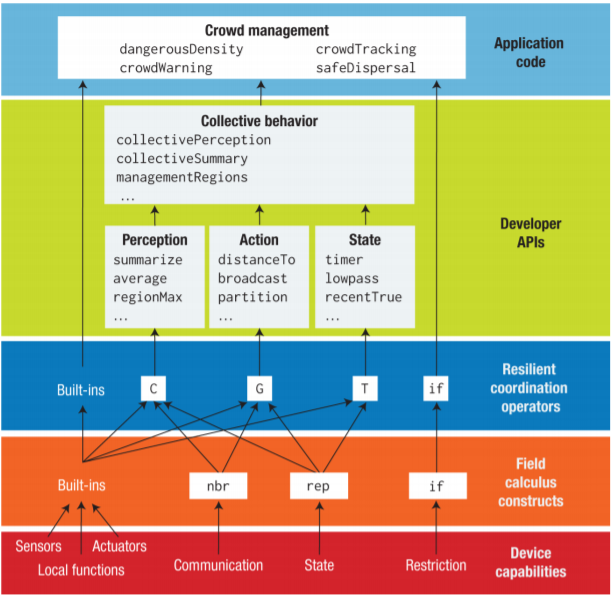
\includegraphics{figures/ACstack.png}
    \caption{Aggregate programming stack.~\cite{BealIEEEComputer2015}}
    \label{fig:ACstack}
\end{figure}

\subsection{Field-calculus}

Field calculus is a theoretical model that describe a set of primitive to manipulate the concept of \textit{computational field}. A computational field is a distributed data structure that maps every networked device to some local value. In field calculus everything is a field (value, variable, expression, function) and the constructs to build and manipulate it are:
\begin{itemize}
    \item \textbf{Functions}, $b(e1,...,e_n)$ applies function $b$ to arguments $e1,...,e_n$. The output field is obtained by the point-wise evaluation of the operator to the input fields.
    \item \textbf{Stateful computation}, $rep(x \leftarrow v)~\{s1; ... ; s_n\}$ a local variable $x$ is defined and initialized to value $v$. Then the value is periodically updated with the result of statements $s1; ... ; s_n$.
    \item \textbf{Interaction}, $nbr(s)$ share the local value of $s$, represented as a field, with the neighbors. The result is a field of fields (the same information shared from the neighbors) that is possible to reduce to a simple field using \textit{hood} operators. 
    \item \textbf{Domain restriction}, $if(e)~\{s1; ... ; s_n\}~else~\{s'_1; ... ; s'_n\}$ split the field in two sub-field according to the evaluation of $e$. Where $e$ is true is applied the statement $s1; ... ; s_n$, while where $e$ is false is applied the statement $s'_1; ... ; s'_n$
\end{itemize}

The behavior of aggregate systems can be expressed as a functional composition of operators that manipulate (evolve, combine, restrict) computational fields~\cite{type-sound}. \todo[inline]{parlare di higher-order field calculus?}

\subsection{Building blocks operators}
Basic field calculus constructors are low level operators and led to an error prone programming. In order to limit the use of this operators,~\cite{buildingBlock} present the set of building block that compose the central layer of the aggregate programming stack, \autoref{fig:ACstack}. This functionalities are then available as library function defined on top of the low level operators. The principal functions presented are:

\begin{itemize}
    \item $G(source, init, metric, accumulate) \rightarrow$ function to spreading information across space. First build a field of shortest path that start from $source$ with the chosen $metric$. Then spread the information across the field starting from the $init$ value and modifying it at each step whit the $accumulate$ function
    \item $C(potential, reduce, local, null) \rightarrow$ function to accumulates $local$ value along the $potential$ field until the source. The final value is obtained applying the $reduce$ function to the $local$ value of the crossed nodes. If there is nothing to accumulate is returned the default value $null$
    \item $T(init, zero, decay)  \rightarrow$ function to evolve the state for a specified period. The period start from $init$ and decrease until $zero$ with a $decay$ rate.
    \item $S(grain, metric)  \rightarrow$ function to split the network in partitions of nodes. This function uses the $metric$ function to define the sets of nodes of size $grain$ and elects a leader for each partition.
\end{itemize}

Reduce the possibility to make mistake with low-level operators is not the only advantage in using this building block, but this functions are also complementary and combining them differently is possible to implement all the principal coordination patterns for distributed system. Finally, an other advantage is that these functions are self-stabilizing and consequently systems build on top of these functions will be self-stabilizing. In complex system, self-stabilizing property guarantee that after each transitory phase, the system return to a stationary state, where is possible predict its behaviour.


\subsection{Protelis}


% linguaggio per field calculus, supporta HFC, inspirato a proto, completamente funzionale, sintassi Java-like, completa interoperabilità con il mondo java, fornisce supporto per tutto lo stack AC, ExecContext e NetManager, esegue su JVM così da garantire interoperabilità


\section{LoRaWAN}
% (what is and network architecture)
LoRaWAN~\cite{loraalliancetechnicalcommittee2020} is a network protocol optimized for long-range communication with low energy consumption, but with the drawback of short and not frequent messages.

A LoRaWAN network, \autoref{fig:LoRaNetwork}, is composed of three fundamental elements: end-device (aka motes), gateway (aka concentrators) and a network-server. 
% 
The topology of the network typically is a star-of-stars topology with the gateway that intermediate between motes and network-server.
% 
The communication between gateway and network-server is IP-based, while the communication between gateway and motes use the LoRa (Long Range) protocol.

\begin{figure}[h]
    \centering
    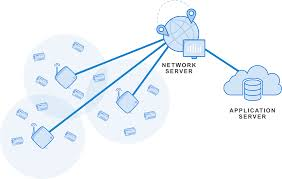
\includegraphics{figures/lora_architecture2.png}
    \caption{LoRaWAN network architecture~\cite{muntasirjoarder2020} with all the fundamental elements. Straight line represent IP-based communication, while the circle around the gateways is the communication range with LoRa protocol.}
    \label{fig:LoRaNetwork}
\end{figure}

The role of the network-server is to govern and optimize the interactions between motes and gateway and provide the mote's packet to the applications in the application server.
% 
So among other tasks, it has to filter duplicated packet received from gateways and find the best gateway to deliver an application message to a mote.
% 
The LoRaWAN protocol, \autoref{fig:LoRaStack}, is composed of two layers: the  physical layer and the MAC one.

\begin{figure}[h]
    \centering
    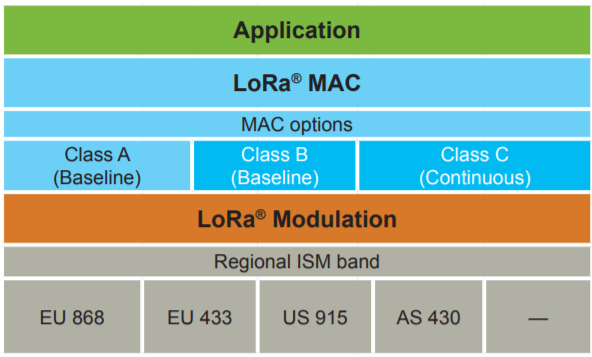
\includegraphics{figures/loraStack.png}
    \caption{LoRaWAN protocol stack~\cite{loraalliance2020} where brown rectangle represent the physical layer and the azures rectangles the MAC one.}
    \label{fig:LoRaStack}
\end{figure}

\subsection{Physical Layer}
The physical layer is based on the LoRa protocol that allows communication until 15 Km of distance, with a data rate from 0.3 Kb/s to 11 Kb/s with LoRa modulation, and to 50 kb/s with FSK modulation.
% 
The most important parameters for the LoRa modulation are Bandwidth (BW), Spreading Factor (SF) and the Code Rate (CR).
% 
The SF value is in the range from 7 to 12 and represents the number of bits in each symbol.
% 
It is an important parameter because define: the maximum packet length, the range of communication and the bit rate.
% 
SF7 means longest packet length and higher bit rate, but shortest communication range; while SF12 means shortest packet length and lower bit rate, but longest communication range.
% 
Another important aspect on SF is that concurrent transmission (from different motes), but with different SF will not produce any collision between the two transmission.
% 
Finally, LoRa uses the regional Industrial, Scientific and Medical (ISM) band.

\subsection{MAC Layer}
% (Class A, B and C)
The aim of this layer is to regulate communication between motes and gateways.
% 
Uplink communication (mote to gateways) uses an ALOHA-like protocol, with motes that start a broadcast communication when they need without checking that the channel is free but applying a small random delay.
% 
For downlink communication (gateways to mote) in order to reduce the battery consumption of the motes and respect latency requirement of different applications, it defines three different classes of device (A, B and C).
% 
Devices of class A define two fixed receiving windows after each uplink communication, with the second one opened only if the mote receives a communication during the first. 
% 
This class has the lowest battery consumption with the drawback of the highest latency. 
% 
Devices of class B allow to define more receive windows, but it is necessary to keep motes and server synchronized via synchronized Beacon. 
% 
This class has a lower latency than class A but also a higher battery consumption. 
% 
Finally, devices of class C allow always to receive messages except when they execute an uplink communication. 
% 
This class has the lowest latency with the drawback of the highest battery consumption.

\section{DingNet: a LoRa-over-MQTT network and simulator}
LoRaWAN protocol not standardize communications after the gateways, but define only that are IP-based.
% 
LoRa-over-MQTT identifies a network where the communication between gateways and network-server is implemented using the public-subscribe pattern via MQTT protocol, and the application server provides data to applications in different ways, but at least via MQTT.
% 
An example of LoRa-over-MQTT architecture is ChirpStack\footnote{\href{https://www.chirpstack.io/}{https://www.chirpstack.io/} (Jan 2020)}, see \autoref{fig:ChirpStack}, that is an open-source LoRaWAN Network Server stack to manage all the LoRaWAN network components and provide data to applications in different ways.

\begin{figure}[h]
    \centering
    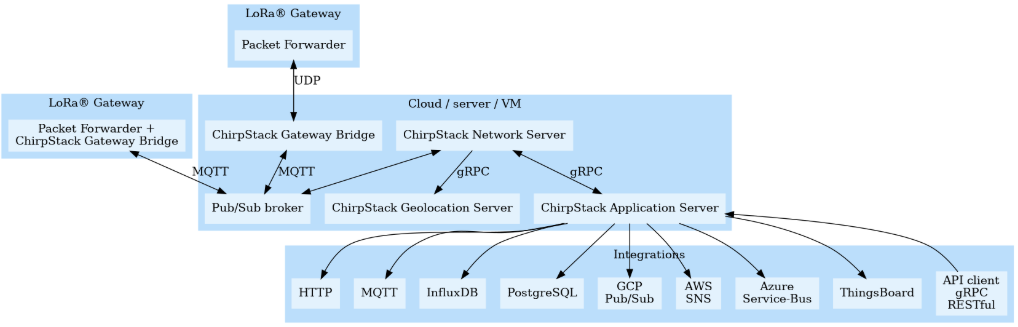
\includegraphics[width=\textwidth]{figures/chirpstack.png}
    \caption{Example of the LoRa-over-MQTT architecture of ChirpStack.~\cite{chirpstack2020}}
    \label{fig:ChirpStack}
\end{figure}

DingNet\footnote{\href{https://admin.kuleuven.be/icts/english/services/dingnet}{https://admin.kuleuven.be/icts/english/services/dingnet} (Jan 2020)} is a real LoRaWAN network composed of 11 gateways that cover the entire university city of Leuven and adopt a LoRa-over-MQTT architecture. 
% 
DingNet allows adding user's devices and applications to the network for research porpoise.
% 
Last year was introduced the DingNet Simulator~\cite{inproceedings} to allow simulation of application in different scenarios before deploying it in the real network to reduce costs and time for the deploy.
% 
It is a time-driven simulator focused on the simulation of LoRa communications between gateways and mote while the rest of the network is simulated whit a high-level abstraction. 
% 
The simulator allows configuring the environment of the network in terms of the position of gateways, motes, and typology of areas that compose the environment. 
% 
Exist different types of areas (like forest, open space, building area) to represent different kinds of areas present in a city; where each area differs for how much decrease the power of a transmission. For example, a building area decreases power more than an open space one.
% 
Motes can be stationary, but also mobile.
% 
For each mote is possible to configure all the most important parameters for a LoRa transmission, like bandwidth, spreading-factor and transmission power. 
% 
The simulator for each transmission computes the time-on-air based on the previous parameters and the size of the packet. 
% 
Then it applies an algorithm to decrease the power of the transmission based on the distance from the source and the typology of the area that the transmission is going through to find all the gateway that will receive the transmission with enough power.
% 
Every transmission is considered arrived to a gateway when is pass enough time (time-on-air) from the beginning of the transmission. 
Then gateway applies a particular algorithm to check if the transmission is collided with others. If not it publishes the received packet on a MQTT broker for the applications.
%
At the end of each simulation is possible to export different information for mote's transmission:
\begin{itemize}
    \item received power from the gateways (dBm)
    \item time on air (ms)
    \item used power for the transmission (dBm)
    \item used energy for the transmission (mJoule)
    \item collision with others transmissions (true/false)
\end{itemize}
% esempi di applicazioni simulate
Nowadays the simulator is used mainly to simulate self-adaptive applications in large scenarios to increase the number of transmission correctly delivered to at least one gateway end reduce the energy consumption of the motes.
